%! Author = manuel
%! Date = 12.05.21

% Preamble
\documentclass[12pt,a4paper]{article}

% https://papers.nips.cc/paper/2017/file/68a9750337a418a86fe06c1991a1d64c-Paper.pdf
% https://arxiv.org/pdf/2006.05990.pdf

% Packages
\usepackage{amsmath}
\usepackage{float}
\usepackage[hscale=0.8,vscale=0.8]{geometry}
\usepackage{amsfonts}
\usepackage{graphicx}


% Document
\begin{document}
    \begin{center}
        Project 3
        \\
        \vspace{0.5cm}
        \textbf{\Large Multi-Agent Actor-Critic Deep Reinforcement Learning}
    \end{center}


    \section{Overview}\label{sec:overview}
    The goal of this project is to train two agents that play tennis.
    The agents receive a reward of +0.1 if they play the ball over the net.
    If they drop the ball they receive a reward of -0.01.
    The score is calculated based on the total cumulative reward both agents get.
    Thus, the agents are trained to work cooperatively rather than competitive.
    \\
    For training I used the MADDPG (Multi Agent Deep Deterministic Policy Gradient).
    I used two separate actor-critic agents that share a replay buffer, and their actor network.
    \\
    The state space consists of eight variables corresponding to the position and velocity of the ball and racket.
    Each agent revives its own, local observation.
    The action space consists of two continuous actions corresponding to movement in direction of the net and vertical direction of the racket.


    \section{Results}\label{sec:results}
    Initially I had a hard time training the two agents because one agent was always way better than the other agent.
    This also had a negative performance on the better agent, since they are trying to optimize a collaborative score.
    After using the same actor network I got way better results and was able to solve the environment in 1638 episodes.

    \begin{figure}[H]
        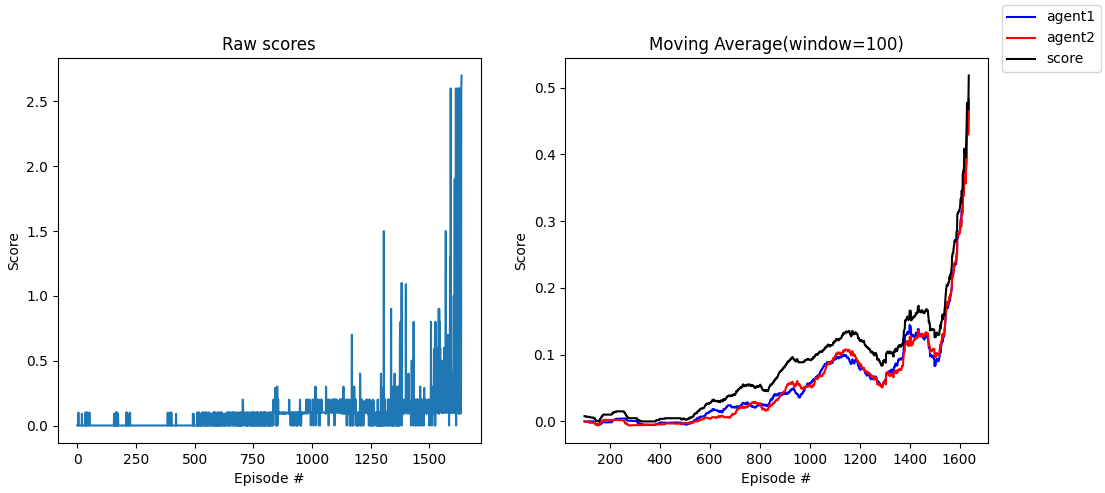
\includegraphics[width=\linewidth]{img/scores1}
        \caption{Scores that the agents achieved per episode}
        \label{fig:scores}
    \end{figure}
    \pagebreak
    I achieved these scores using the following \textbf{hyper parameters}:
    \begin{center}
        \begin{tabular}{||l c l||}
            \hline
            Parameter    & Value      & Description \\ [0.5ex]
            \hline\hline
            gamma        & 0.994      & discount factor                                                           \\
            \hline
            lr\_actor    & 0.001      & learning rate of the actor network                                        \\
            \hline
            lr\_critic   & 0.0005     & learning rate of the critic network                                       \\
            \hline
            tau          & 0.001      & update factor for soft update                                             \\
            \hline
            buffer\_size & $1*10^{6}$ & Size of the experience replay buffer                                      \\
            \hline
            batch\_size  & 150        & minibatch size (how many samples are drawn from the buffer when learning) \\
            \hline
        \end{tabular}
    \end{center}

    The actor networks of both agents had one hidden layer with 64 input features and 64 output features.
    The critic networks of both agents had one hidden layer with 102 input features and 100 output features


    \section{Ideas for future improvements}\label{sec:ideas}
    I could improve the learning of the individual DDPG Agents by using algorithms like REINFORCE or Rainbow.

\end{document}